% !TEX TS-program = pdflatex
% !TEX encoding = UTF-8 Unicode

% This is a simple template for a LaTeX document using the "article" class.
% See "book", "report", "letter" for other types of document.

\documentclass[11pt]{article} % use larger type; default would be 10pt

\usepackage[utf8]{inputenc} % set input encoding (not needed with XeLaTeX)

%%% Examples of Article customizations
% These packages are optional, depending whether you want the features they provide.
% See the LaTeX Companion or other references for full information.

%%% PAGE DIMENSIONS
\usepackage{geometry} % to change the page dimensions
\geometry{a4paper} % or letterpaper (US) or a5paper or....
% \geometry{margin=2in} % for example, change the margins to 2 inches all round
% \geometry{landscape} % set up the page for landscape
%   read geometry.pdf for detailed page layout information

\usepackage{graphicx} % support the \includegraphics command and options

% \usepackage[parfill]{parskip} % Activate to begin paragraphs with an empty line rather than an indent

%%% PACKAGES
\usepackage{booktabs} % for much better looking tables
\usepackage{array} % for better arrays (eg matrices) in maths
\usepackage{paralist} % very flexible & customisable lists (eg. enumerate/itemize, etc.)
\usepackage{verbatim} % adds environment for commenting out blocks of text & for better verbatim
\usepackage{subfig} % make it possible to include more than one captioned figure/table in a single float
\usepackage{amsmath}

% These packages are all incorporated in the memoir class to one degree or another...

%%% HEADERS & FOOTERS
\usepackage{fancyhdr} % This should be set AFTER setting up the page geometry
\pagestyle{fancy} % options: empty , plain , fancy
\renewcommand{\headrulewidth}{0pt} % customise the layout...
\lhead{}\chead{}\rhead{}
\lfoot{}\cfoot{\thepage}\rfoot{}

%%% SECTION TITLE APPEARANCE
\usepackage{sectsty}
\allsectionsfont{\sffamily\mdseries\upshape} % (See the fntguide.pdf for font help)
% (This matches ConTeXt defaults)

%%% ToC (table of contents) APPEARANCE
\usepackage[nottoc,notlof,notlot]{tocbibind} % Put the bibliography in the ToC
\usepackage[titles,subfigure]{tocloft} % Alter the style of the Table of Contents
\renewcommand{\cftsecfont}{\rmfamily\mdseries\upshape}
\renewcommand{\cftsecpagefont}{\rmfamily\mdseries\upshape} % No bold!

%%% END Article customizations

%%% The "real" document content comes below...

\title{FMAN20 - Assignment 1}
\author{Santhosh Nadig}
%\date{} % Activate to display a given date or no date (if empty),
         % otherwise the current date is printed 

\begin{document}
\maketitle

\section{}
The image matrix is given by
\begin{equation}
f = 
\begin{bmatrix}
         0  &  11.25 & 15 &  11.25   &      0 \\
         0  & 11.25 &  15 &  11.25   &      0 \\
         0  & 11.25 &  15 & 11.25    &     0 \\
         0  & 11.25 &  15 &  11.25   &      0 \\
         0  & 11.25 &  15 &  11.25    &     0 \\
\end{bmatrix}
\end{equation}
\section{}

\section{}

\section{}
\subsection{Scalar Product}
The scalar product of two images  $f$ and  $g$ is defined as
\begin{equation}
f \cdot g = \sum_{i=0}^M \sum_{j=0}^N f(i,j) g(i,j) .
\end{equation}
\subsection{Norm}
The norm of an image  $f$ is defined as
\begin{equation}
\| f \| = (f^* \cdot f)^{1/2} .
\end{equation}
\section{}

\section{}

\section{}

The MATLAB code for segmentation (\texttt{im2segment.m}) is listed below:
\begin{verbatim}
function [S] = im2segment(im)
% [S] = im2segment(im)

nrofsegments = 4;
m = size(im,1);
n = size(im,2);

% Thresholding algorithm. Set all 'pixels' < T = 0
% This improves contrast.
T=220;
im2 = im; im2(im2 < T) = 0;
% Invert the pixels (convert white -> black & black -> white)
im2 = not(im2)*255;

% Find the start and end of the entire group
% start_idx: Start of the characters
% end_idx  : End of the characters
% sum of a column of pixels exceeds 'threshold' => separation
threshold = 255*m*0.965;
row_sum = sum(im,1);
start_idx = find(row_sum < threshold, 1);
end_idx = n - find(fliplr(row_sum) < threshold, 1);
% row_sum = 1 where characters are present. Otherwise, its zero.
row_sum = row_sum(start_idx:end_idx) < threshold;

% Find each of the individual characters
segment_start=1;
for kk = 1:nrofsegments;
    segment_end = segment_start + find(row_sum(segment_start:end) < 1,1) - 1;
    temp = zeros(m,n); 
    temp_idx = start_idx +(segment_start:segment_end);
    temp(:,temp_idx) = im2(:,temp_idx);
    S{kk} = temp;
    segment_start = segment_end + find(row_sum(segment_end:end)>0,1) - 1;
end;
segment_end=length(row_sum);
temp_idx = start_idx +(segment_start:segment_end);
temp = zeros(m,n);
temp(:,temp_idx) = im2(:,temp_idx);
S{kk+1} = temp;
\end{verbatim}

The result from benchmarking script is listed below:
\begin{verbatim}
>> inl1_test_and_benchmark
You tested 10 images in folder ../datasets/short1
The jaccard scores for all segments in all images were
    0.8211    0.8288    0.8980    0.8794    0.9008
    0.8631    0.7823    0.8652    0.7886    0.9851
    0.8611    0.8881    0.8525    0.7965    0.8611
    0.7876    0.8131    0.8737    0.8378    0.9531
    0.8631    0.8632    0.7736    0.8824    0.8721
    0.9029    0.7857    0.8904    0.8000    0.8814
    0.8721    0.8706    0.7823    0.8552    0.8925
    0.7876    0.9778    0.8690    0.8689    0.8537
    0.9028    0.8889    0.7799    0.8630    0.7736
    0.8611    0.9683    0.7895    0.8673    0.9029

The mean of the jaccard scores were 0.85756
You can do better
\end{verbatim}

\begin{figure}
\centering
\subfloat[OCR to be segmented]{
  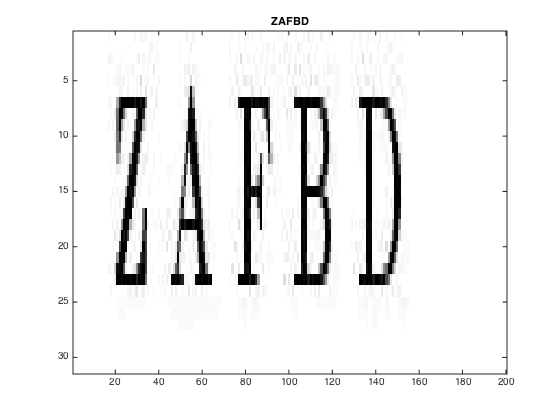
\includegraphics[width=65mm, height=15mm]{zafbd.png}
}
\subfloat[Segment 1]{
  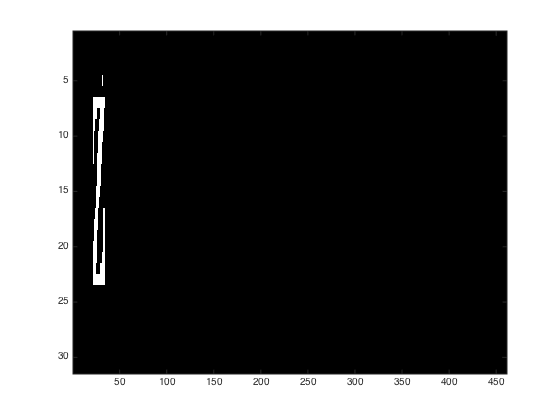
\includegraphics[width=65mm, height=15mm]{z.png}
}
\hspace{0mm}
\subfloat[Segment 2]{
  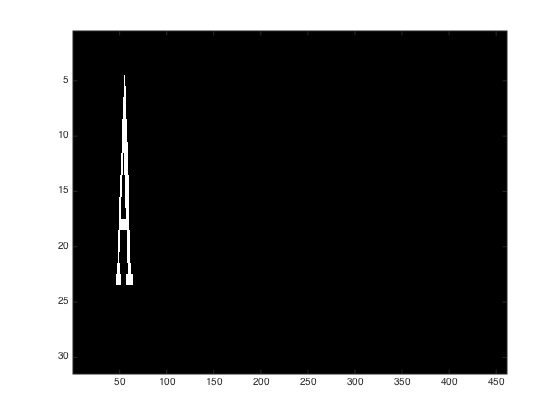
\includegraphics[width=65mm, height=15mm]{a.png}
}
\subfloat[Segment 3]{
  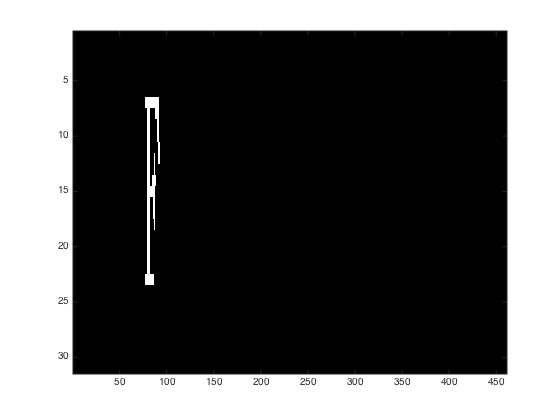
\includegraphics[width=65mm, height=15mm]{f.png}
}
\hspace{0mm}
\subfloat[Segment 4]{ 
  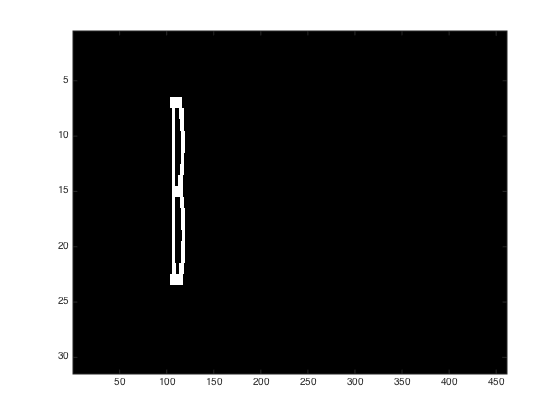
\includegraphics[width=65mm, height=15mm]{b.png}
}
\subfloat[Segment 5]{
  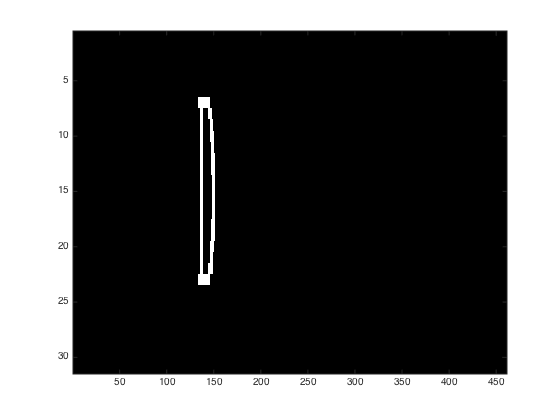
\includegraphics[width=65mm, height=15mm]{d.png}
}
\caption{Result of im2segment}
\end{figure}

\section{}

\end{document}
